%*************************************************************
\chapter{Kollaboratives Design}\label{ch:kollaborativesDesign}
%*************************************************************

Kollaborative Aktivitäten sind ein wichtiger Anwendungsbereich für elektronische Technologien \citep{Kvan:2000}. Designer arbeiten immer häufiger nicht mehr alleine für sich, sondern mit anderen Designern, aber auch Leuten aus anderen Disziplinen zusammen. Da komplexe Probleme mehr Expertise und Wissen erfordern, als eine einzelne Person haben kann, sind Teilnahme, Kommunikation und Kollaboration seitens aller involvierten Akteure notwendig. Die intellektuelle, kulturelle und soziale Vielfalt, die dem Projekt dadurch zugutekommt, ist eine wichtige Quelle für soziale Kreativität \citep{Fischer:2005}. 

\medskip Für das Verständnis von kollaborativem Design ist es wichtig, die Bedeutung von Kollaboration zu erörtern. Betrachten wir dazu die verschiedenen Aktivitäten, die gemeinhin unter dem Begriff Kollaboration zusammengefasst werden. Zur Lösung von gegebenen Problemen, beispielsweise dem Design eines neuen Produkts, bilden Individuen Teams und Gruppen, um vom sogenannten >>process gain<< \citep{steiner:1972} zu profitieren. Von kollaborativem Erfolg kann dann gesprochen werden, wenn die Gruppe etwas erreicht, das ihre  Mitglieder alleine nicht hätten erreichen können \citep{Kvan:2000}. Kollaboration kann als gemeinsames Lösen von Problemen verstanden werden: Individuen haben ein oder mehrere gemeinsame Ziele und arbeiten zusammen, um befriedigende Lösungen zu finden. Thomas Kvan definiert den Begriff Kollaboration durch Bezugnahme auf auf das Oxford Englischwörterbuch:

\begin{quote} 
	>>Indeed, the Oxford English Dictionary de- fines collaborate as ‘‘to co-operate, especially in literary, artistic or scientific work’’, deriving from the Latin words \emph{col labore}, to work along side one another.<< \citep{Kvan:2000} 
\end{quote} 

Weiters schreibt er, dass kollaboratives Design eine weitaus anspruchsvollere Aktivität ist, als einfach nur ein Projekt in einem Team abzuschließen. Es muss ein gemeinsames, ganzheitliches und kreatives Resultat produziert, nicht bloß eine gewisse Arbeit erledigt werden \citep{Kvan:2000}.

Viele Arten von Design können nicht von einem einzelnen Designer gehandhabt werden. Im Bereich Architektur arbeiten beispielsweise sehr viele Leute aus verschiedenen Disziplinen zusammen, um ein Gebäude zu entwerfen. 

HIER NOCH WEITER SCHREIBEN: COLLABORATIVE DESIGN WHAT IS IT?

\section{Soziale Aspekte \& Probleme} 

Kollaboratives Design von mehreren Personen aus verschiedenen beruflichen Disziplinen birgt sehr viele und komplexe soziale Aspekte. Jede dieser Personen hat einen eigenen Charakter, verschiedene kulturelle, soziale und politische Ansichten und vor allem eigene Interessen und Sichtweisen.

\autoref{fig:kilkerTree} zeigt den sogenannten >>Tree Swing<<\footnote{zu Deutsch: Baumschaukel} Sketch, der auf witzige Weise die Problematik von kollaborativem Design aufzeigt. Man sieht darin die verschiedenen Visionen einer Baumschaukel der jeweiligen Teammitglieder. Jede einzelne Darstellung der Schaukel stereotypisiert eine ins Projekt involvierte Rolle \citep{Kilker:1999}.

\medskip Designprojekte im technologischen Bereich umfassen immer mehr Teammitglieder aus unterschiedlichen Berufsgruppen. Egal ob diese Personen in einem Meeting zusammensitzen oder ihre Arbeit via Videokonferenz erledigen, sie alle haben verschiedne Perspektiven auf das Projekt, die Anforderungen und die Lösung. Jeder muss seine eigene Sichtweisen argumentieren und versuchen so gut wie möglich durchzusetzen, ähnlich dem Sketch in \autoref{fig:kilkerTree}. Julian Kilker bezeichnet diese verschiedenen Rollen als >>design identities<<\footnote{zu Deutsch: Designidentität}. Jede dieser >>design identities<< hat eine eigene Meinung, eigene Standpunkte und eine eigene Einstellung gegenüber Technologie und Design. All diese Faktoren beeinflussen das Design, den Prozess und das Endprodukt der Projektarbeit \citep{Kilker:1999}.

\begin{figure}
	{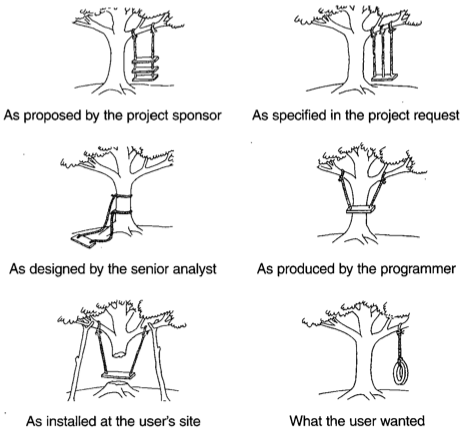
\includegraphics[width=1\linewidth]{gfx/kilkerTreeSwing}}
\caption[Tree Swing Sketch \newline \citep{Kilker:1999}]{Der >>Tree Swing<< (Baumschaukel) Sketch zeigt die Fallen, in die man bei kollaborativem Design laufen kann. Wenn jeder eine andere Vorstellung vom Produkt hat, dann leidet das Endresultat.}\label{fig:kilkerTree}
\end{figure}

\medskip Die Theorie der sozialen Identität ist eine sozialpsychologische Perspektive, die erläutert, wie Menschen soziale Identitäten (beispielsweise >>Entwickler<<, >>Manager<< oder >>Programmierer<<) annehmen, halten und verwenden \citep{Hogg:1988}.

Aufbauend auf Sherifs Untersuchungen der realistischen Konflikttheorie \citep{Sherif:1966}, ist die Theorie der sozialen Identität nützlich für die Erforschung der Art und Weise, wie Individuen in Gruppen zusammenarbeiten \citep{Kilker:1999}. Personen sind Teil einer sozialen Gruppe, wenn sie eine gemeinsame Definition ihrer selbst als Teil dieser Gruppe vertreten \citep{Hogg:1988}.

Sherif hat Konflikte in Gruppen und Teams ausgiebig untersucht. Dabei hat er für seine Zwecke die Testpersonen so in Gruppen aufgeteilt, dass ein möglichst kompetitives Klima innerhalb des jeweiligen Teams entstand \citep{Sherif:1966}. Die Theorie der sozialen Identität fokussiert im Gegensatz zu diesen designierten Teams auf möglichst realistische Gruppenkonstellationen.

\medskip Idealisierte soziale Identitäten spielen bei Interaktionen innerhalb einer Gruppe eine wichtige Rolle. Menschen brauchen sie, um sich selbst und andere zu definieren und Vergleiche herzustellen. Jeder hat ein stereotypes Bild der einzelnen involvierten Berufsdisziplinen im Kopf, basierend auf Bildung und Erfahrung. Der Theorie der sozialen Identität zufolge, betonen Leute im eigenen Team Ähnlichkeiten zwischen sich und den Kollegen, gegenüber anderen Gruppen heben sie jedoch Unterschiede hervor. Generell kommen stereotype Sichtweisen eher in multidisziplinären (heterogenen) Teams zum Vorschein, als in homogenen Konstellationen.

\medskip Im sozialen Wettbewerb tendieren soziale Identitäten zur Polarisation. Die Individuen ordnen sich und den anderen eine gewisse Identität und dessen Ideale zu und kategorisieren damit jeden in der Gruppe. Solche polarisierenden Identitäten sind beispielsweise Liberale oder Konservative in politischer Hinsicht, Vertreter von qualitativen oder quantitativen Methoden in wissenschaftlicher Hinsicht oder die stereotypischen Interpretationen von PC oder Mac Benutzern.

Stereotype sind von Natur aus simplifiziert und stilisiert. Kein Mensch entspricht genau so einem verzerrten Bild, denn jeder hat Ansichten, Ideale und Eigenschaften, die sich davon unterscheiden. 

\medskip Obwohl es im Bereich Design viele unterschiedliche soziale Identitäten gibt, wollen wir uns im Folgenden auf zwei typische Identitäten konzentrieren: eine vertritt Ansichten und Methoden, die technologiezentriert sind und die andere vertritt sozialzentrierte Ansichten und Methoden. Wir prüfen die Kollaboration zwischen diesen zwei Charakteren und die damit verbundenen Implikationen \citep{Kilker:1999}.

Die technologiezentrierte Identität bevorzugt ein gut geplantes, systematisches und lineares Design, das Pahl und Beitz als >>systematischen Ansatz<< bezeichnen \citep{Pahl:1988}, während die sozialzentrierte Identität benutzerzentriertes und partizipatives Design sowie eine iterative Vorgehensweise vorzieht.

\autoref{tab:kilkerIdeals} zeigt die unterschiedlichen, polarisierenden Ideale dieser beiden Designidentitäten nach Kilker \citep{Kilker:1999}. Donald Norman nennt diese auseinander laufenden Perspektiven >>menschenzentriert<< und >>maschinenzentriert<<. Erstere ordnet den Menschen der Maschine über, denn er ist der Maschine durch Kreativität, Einfallsreichtum und Flexibilität überlegen. Computer hingegen sind dumm, einfallslos und starr. Die maschinenzentrierte Perspektive sieht den Menschen dagegen als unorganisiert, emotional und unlogisch, während Maschinen als geordnet, objektiv und logisch betrachtet werden \citep{Norman:1994}. 

\begin{table}
    \myfloatalign
\begin{tabularx}{\textwidth}{p{2.4cm}XX}
    \toprule
	    \tableheadline{Faktor} & \tableheadline{TZI} & \tableheadline{SZI}
	       	\\ \midrule
	
			\small{
				Charakteristiken guten Designs
			} & 
			\small{
				Fokus auf technologische Charakteristiken: Effiziente >>clevere<< Lösung, geringer Instandhaltungsaufwand. Das beste Design kann quantitativ ermittelt werden und das Ziel ist es, dieses zu implementieren
			} & 
			\small{
				Fokus auf soziale Charakteristiken: Funktioniert in der gegebenen sozialen Umgebung und befriedigt die Bedürfnisse der Benutzer. Es gibt mehrere Perspektiven von gutem Design und das Ziel ist es, die beste Kombination zu finden.
			} \\
			\hline %------------------------------------------------------------
			\small{
				Designprozess
			} & 
			\small{
				Systemorientiert, basierend auf Spezifikationen
			} & 
			\small{
				Iterativ, benutzerorientiert. Kollaboration verbessert Design.
			} \\
			\hline %------------------------------------------------------------
			\small{
				Verantwortung der Designer
			} & 
			\small{
				Designer sind nicht verantwortlich für soziale Verwendung von Technologie, die Verantwortung liegt beim Benutzer.
			} & 
			\small{
				Designer sollen den sozialen Kontext der Technologie berücksichtigen.
			} \\
			\hline %------------------------------------------------------------
			\small{
				Die Rolle von Evaluierung in Design
			} & 
			\small{
				Quantitativ: gibt an, ob die Implementierung die Anforderungen der Spezifikation erfüllt. Benutzer gehen nicht rein logisch vor, ihre Evaluierung ist oft widersprüchlich und bringt wenig.
			} & 
			\small{
				Qualitativ und ethnographisch: zeigt Diskrepanzen zwischen Spezifikation und Bedürfnissen der Nutzer auf. Die Benutzer haben höchste Priorität und sollten deshalb in den Designprozess einbezogen werden.
			} \\
			\hline %------------------------------------------------------------
			\small{
				Wie wird das andere Ideal wahrgenommen?
			} & 
			\small{
				Sozialzentrierten Idealen fehlt es an konkreten Zielen. Befürworter verlangen oft substanzielle Designänderungen aufgrund von Trivialitäten.
			} & 
			\small{
				Technologiezentrierte Ideale sind starr und unflexibel. Befürworter sind zwar technisch kompetent, weigern sich aber, soziale Aspekte zu berücksichtigen.
			}
			\\ \bottomrule
\end{tabularx}
  \caption[Polarisierende Designideale \newline \citep{Kilker:1999}]{Die unterschiedlichen Designideale von technologiezentrierten und sozialzentrierten Identitäten. \\TZI = Technologiezentriertes Ideal \\SZI = Sozialzentriertes Ideal}
  \label{tab:kilkerIdeals}
\end{table}

\medskip Neben der stereotypischen Sichtweise der Kollegen im Projekt, hat auch jeder Designer ein stereotypisches Bild vom designierten Endbenutzer. Problematisch ist jedoch bereits die Begrifflichkeit >>der (End)benutzer<<, da Technologien von sehr vielen und sehr unterschiedlichen Individuen aus verschiedenen Kontexten benutzt werden \citep{Agre:1995}. Daher muss der Begriff >>Benutzer<< explizit und implizit während des Designprozesses erörtert und ein authentisches Bild vom tatsächlichen Endbenutzer geschaffen werden. Designer können dies direkt durch Diskussion mit und Observation von potenziellen Nutzern oder indirekt und hypothetisch durch Stereotypisierung von Szenarios und Fallstudien erreichen.

\medskip Eine hypothetische Benutzergruppe wäre beispielsweise der >>naive user<<, der laut Annahme der Technologie komplett fremd ist. Technologiezentriertes Design würde davon ausgehen, dass dieser Benutzer in der selben Welt wie der Programmierer lebt und dass rationale und formale Methoden eingesetzt werden können, um die Interaktionen zwischen diesem Menschen und der Maschine zu modellieren. Das Gegenlager, sozialzentriertes Design, würde mit der Annahme starten, technische Systeme könnten nicht ohne ein umfassendes Verständnis des sozialen Kontexts entwickelt werden und die Zielgruppe müsste aktiv auf die neue Technologie vorbereitet werden.

\medskip Soziale Identitäten sind in zweierlei Weisen eine Herausforderung bei der Kollaboration in einem Team: zum einen ist es für die involvierten Personen schwierig, ihre unterschiedlichen Perspektiven und Meinungen zu vereinbaren, und zum anderen hat auch jeder der Beteiligten eine andere Vorstellung davon, wie der Designprozess und die Kollaboration selbst ablaufen sollen.

Jeder Mensch ist immer Teil von mehreren sozialen Gruppen. In einem kollaborativen Designkontext ist jeder ein Teil des Projektteams und zusätzlich noch Teil seiner Berufsgruppe und den damit verbundenen sozialen Kontext. Der Zwiespalt zwischen diesen beiden Gruppen kann dazu führen, dass die Qualität der Zusammenarbeit leidet. Wenn Teammitglieder zu sehr die Rolle ihrer Berufsgruppe einnehmen, kann das in festgefahrenen Diskussionen resultieren \citep{Kilker:1999}. Wird hingegen die Identität als Teammitglied zu sehr in den Vordergrund gerückt, kann dies dazu führen, dass die eigene Perspektive nicht mehr genügend eingebracht und dadurch wertvoller Input verloren geht \citep{Irving:1982}.

Sherif hat durch seine Forschung herausgefunden, dass die Kollaboration zwischen polarisierenden Identitäten durch die Einführung eines gemeinsamen Gegners, oder schärfer gesagt, durch die Einführung eines Feindes angekurbelt werden kann. Besser ist es hingegen, übergeordnete Ziele für die Gruppe einzuführen, deren Erreichung für das Team äußerst reizvoll ist und die für das einzeln Individuum absolut unerreichbar sind \citep{Sherif:1966}.

Viele Mitglieder in Designteams sind in kollaborativem Arbeiten ungeübt. Dieses Problem rührt daher, dass technische Ausbildungen darauf abzielen, optimale Lösungen zu finden, anstatt auch Kompromisse und Mittelwege in Betracht zu ziehen. Sozialzentrale Ausbildungen lehren hier eine andere Vorgangsweise. Sie propagieren in kollaborativer Arbeit auch zu diskutieren und zu verhandeln, das technologiezentrierte Lager empfindet diese Methoden hingegen als ineffektiv. Wir wollen dazu einen beispielhaften Kommentar aus einer Online-Gruppendiskussion über Hypertextstandards\footnote{Unter Hypertext wird in der Regel ein Text mit aktivierbaren Elementen verstanden, die im einfachsten Fall dazu dienen, direkt zu anderen Stellen im Text oder zu anderen Texten zu springen} betrachten, in dem er sich für seinen harschen Tonfall in einer vorhergehenden Aussage rechtfertigt:

\begin{quote}
	>>I try to discourage what I see as bad practice, I'm stronger about it here because I think we're alle technical people, I know as an engineer I much prefer direct talk to soft sell. And my experience is most engineers aren't overly sensitive - they can take heat as well as give it without making it a personal issue.<<\footnote{zu Deutsch: >>Ich versuche immer von schlechten Methoden abzuraten. Ich tue das in dieser direkten Form, weil ich denke wir sind hier Techniker unter uns. Als Ingenieur bevorzuge ich, Dinge direkt und konkret anzusprechen und meine Erfahrung hat mir gezeigt, dass die meisten Ingenieure nicht sonderlich zimperlich oder sensibel sind. Sie können hitzige Diskussionen genauso gut verdauen, wie anzetteln. Keiner nimmt das persönlich.<<} \\\citep{Kilker:1999}
\end{quote}

Aus dieser Perspektive betrachtet wirkt der sozialzentrierte Designprozess ineffizient. Soziale Interaktionen sollten direkt, effizient und vernünftig sein, um technische Probleme zu lösen. Ein guter Ingenieur muss dieser Ansicht nach Kritik einstecken können, um zur optimalen technischen Lösung zu gelangen. 

\medskip Es wird klar, dass Mitglieder eines heterogenen Designteams sich nicht nur durch ihre Designidentitäten, sondern auch durch ihre Kollaborationstechniken unterscheiden. Konflikte sind daher vorprogrammiert und einige davon sind auch tatsächlich hilfreich. Sind die Ideale jedoch zu verschieden und lassen sich nicht vereinbaren, leidet der Designprozess und folglich die Qualität des Produkts \citep{Kilker:1999}. 

\section{Analyse eines kollaborativen Designmeetings} 

Nigel und Anita Cross haben Teamwork und implizite soziale Prozesse in einem Experiment untersucht \citep{Cross:1995}. Dazu haben sie ein Team aus drei Personen zusammengestellt und eine Videoobservation durchgeführt. Kerry, Ivan und John arbeiteten alle für die selbe Design-Consulting-Agentur und hatten sehr ähnliche Jobrollen innerhalb dieser Agentur. Sie waren hierarchisch gesehen also alle ungefähr gleichgestellt und brachten keine vordefinierten Rollen mit sich. Aufgabe des Workshops war es, einen Fahrradgepäckträger zu entwickeln. Bei ihrer Analyse konzentrierten sich Nigel und Anita Cross auf die folgenden Kernpunkte:

\begin{itemize}
	\item \nameref{sec:collabRoles}
	\item \nameref{sec:collabActions}
	\item \nameref{sec:collabInformation}
	\item \nameref{sec:collabProblem}
	\item \nameref{sec:collabConcepts}
	\item \nameref{sec:collabConflicts}
\end{itemize}

\subsection{Rollen und Beziehungen}\label{sec:collabRoles}

Die Untersuchungen haben ergeben, dass im Team verschiedene Rollen eingenommen wurden. Teilweise wurden Rollen durch das Team geformt und zugewiesen, andere potenzielle Rollen wurden vom Team ignoriert und konnten sich dadurch nicht vollständig entwickeln. Die nachfolgenden Auszüge aus dem Transkript zeigen die Entwicklung und Festigung von Rollen und Beziehungen zwischen den Teammitgliedern.

\medskip Nach dem Lesen der Anforderungen schlägt Kerry vor damit zu beginnen, das Design des bestehenden Prototypen zu analysieren.

\begin{extract}[Kerry schlägt vor, den bestehenden Prototypen zu reviewen.]
	{
		\myfloatalign
		\begin{tabularx}{\textwidth}{p{1cm}X}
    		Kerry & what do we need? I guess we should look at their existing prototype, huh?
		\end{tabularx}
	}
	\captionX{Vorschlag von Kerry.}
\end{extract}

John möchte zuerst lieber sicherstellen, dass alle die Problematik korrekt verstanden haben und vom selben reden.

\begin{extract}[John möchte sicherstellen, dass jeder die Problemstellung genau verstanden hat.]
	{
		\myfloatalign
		\begin{tabularx}{\textwidth}{p{1cm}X}
    		John & yeh, em, let me think; we could also just sort of like try to quantify the problem, because - what's your understanding of the problem first of all?
		\end{tabularx}
	}
	\captionX{Johns Sicherstellung.}
\end{extract}

Diese Klärung der Problematik wird dann tatsächlich vom Team durchgeführt. Kerrys Vorschlag wurde somit ignoriert.

\medskip Während dieser Phase der Klärung schlägt Kerry vor, Informationen aus dem Report der Benutzerevaluierung zu nehmen.

\begin{extract}[Kerry weist erneut auf die Evaluierung des bestehenden Prototypen hin.]
	{
		\myfloatalign
		\begin{tabularx}{\textwidth}{p{1cm}X}
    		Kerry & they're not pleased with it so far, and the users' tests have some - in fact it would be nice if we could see those users' tests to em see what the shortcomings were.
		\end{tabularx}
	}
	\captionX{Kerrys Hinweis.}
\end{extract}

Dieser Vorschlag wird von den anderen beiden Teammitgliedern ignoriert. Kurz nachher, während der Ablaufplanung, erwähnt Ivan den Begriff >>Information<< und Kerry weist erneut auf den Report der Benutzerevaluierung und seine Nützlichkeit hin. Wieder erreicht sie die anderen beiden damit nicht und ihre Anregung wird nicht umgesetzt.

\begin{extract}[Erneut wird Kerrys Anliegen von den anderen ignoriert.]
	{
		\myfloatalign
		\begin{tabularx}{\textwidth}{p{1cm}X}
    		Ivan  & information or \\
			Kerry & yeah we wanna look at the em customer feedback or the users' testing \\
			John  & oh-yeah, so maybe, yeah, wherever that comes in in this list...
		\end{tabularx}
	}
	\captionX{Kerrys Anliegen wird ignoriert.}
\end{extract}

Etwas später lenkt Kerry wieder ein und fragt erneut nach dem Report. Diesmal geht Ivan darauf ein.

\begin{extract}[Diesmal hat Kerry Erfolg und Ivan geht auf ihren Vorschlag ein.]
	{
		\myfloatalign
		\begin{tabularx}{\textwidth}{p{1cm}X}
    		Ivan & I think I'd also like to get the information on em \\
			Kerry & the user testing \\
			Ivan & the user testing
		\end{tabularx}
	}
	\captionX{Kerry hat Erfolg.}
\end{extract}

\medskip Nach der Klärungsphase empfiehlt Ivan, einen zeitlichen Ablaufplan festzulegen. John und Ivan beginnen sogleich mit dieser Planung. Ivan beginnt dann, die diversen Dokumente auf dem Tisch auszulegen und zu ordnen und John nützt die Gelegenheit, um Ivan zum Verantwortlichen für die Ablaufplanung zu ernennen. 

\begin{extract}[John schlägt vor, Ivan sollte sich um den zeitlichen Ablauf kümmern.]
	{
		\myfloatalign
		\begin{tabularx}{\textwidth}{p{1cm}X}
    		Ivan & ...let's get this stuff sorted out \\
			John & OK you were talking about schedule stuff before, do you wanna \\
			Ivan & yeah, I think we should uh just figure out \\
			John & just set some time limits for ourselves
		\end{tabularx}
	}
	\captionX{Johns Vorschlag.}
\end{extract}

Etwas später, als Ivan die Planung durchführt, wird diese Rolle nochmals von John bestätigt.

\begin{extract}[John bestätigt Ivan erneut in seiner Rolle.]
	{
		\myfloatalign
		\begin{tabularx}{\textwidth}{p{1cm}X}
    		Ivan & five-thirty we'll move on to the final cost and presentation... let's leave ourselves a little bit of time \\
			Kerry & mm mm \\
			John & Ivan's gonna be Mister Schedule \\
			Ivan & yeah [...] on time, under budget
		\end{tabularx}
	}
	\captionX{Kerry bestätigt Ivan.}
\end{extract}

Ivan hat somit die Rolle des Ablaufplaners übernommen und wird sie für die restliche Sitzung beibehalten.

\medskip Es wird schnell klar, dass Kerry Schwierigkeiten hat, ihre bevorzugte Vorgangsweise durchzusetzen. Ivan scheint mit seiner Rolle als Ablaufplaner recht glücklich zu sein und hat keine Einwände gegen diese Aufgabe. John scheint viel Einfluss darauf zu haben, wie sich die Dinge im Team entwickeln und was gemacht wird. Die Auszüge zeigen die Muster der Rollen und Beziehungen, die sich mehr oder minder durch die gesamte Sitzung ziehen. Trotzdem werden Rollen kurzzeitig getauscht und jeder der drei übernimmt irgendwann einmal die Führung der Gruppe. Jeder verkörpert diese Rolle jedoch auf seine eigene Art und Weise.

Die Autoren weisen darauf hin, dass es nötig wäre, die Analyse weiter fortzuführen und zusätzliche, wichtige Faktoren zu berücksichtigen. Zum einen wäre es interessant zu analysieren, was einzelne Teammitglieder machen, wenn sie sich nicht gerade im Mittelpunkt der Teambeschäftigung befinden. Sie könnten entweder inaktiv sein, dem Geschehen aus einer Distanz beiwohnen, oder parallele Aktivitäten durchführen. Außerdem wäre es wichtig, Körperhaltung, Körpersprache, Gestik und Mimik genauer zu prüfen. Ebenso wichtig bezeichnen sie eine eingehende Analyse von Gelächter und Witzen zur Vermeidung von Konflikten.

\subsection{Planung und Tätigkeiten}\label{sec:collabActions}

Das von Cross und Cross untersuchte Team legte großen Wert auf die Planung von Ablauf und Tätigkeiten. Dies scheint eine logische Vorgangsweise zu sein, aber oft gehen Teams anders an die Sache heran. Gerade in frühen, konzeptionellen Phasen von Design, ist die Arbeit ungeplant, intuitiv und spontan. Designer legen häufig ein sogenanntes opportunistisches Verhalten an den Tag. Das bedeutet, sie unterlassen geplante Aktivitäten und gehen spontanen Ideen nach, sobald sie ihnen einfallen. Im Team kann das aber zu Schwierigkeiten führen, denn die Aktivitäten der einzelnen Mitglieder müssen koordiniert und abgestimmt werden. 

\medskip Die Planungsphase im Team von Kerry, Ivan und John beginnt als Ivan vorschlägt, einen Ablaufplan zu erstellen, anstatt aus dem Stegreif zu agieren.

\begin{extract}[Ivan möchte den Ablauf zuerst planen.]
	{
		\myfloatalign
		\begin{tabularx}{\textwidth}{p{1cm}X}
    		Ivan & should we uh prepare a schedule and then just sorta stick to it, or should we uh just start working? \\
			John & no, it's probably a good idea to try to quantify our amount of time; the kinda time we have left (laugh) \\
		\end{tabularx}
	}
	\captionX{.}
\end{extract}

Ivan und John listen daraufhin die folgenden Aktivitäten auf einem Blatt Papier auf:

\begin{itemize}
	\item Quantifizieren des Problems
	\item Konzepte generieren
	\item Konzepte verfeinern
	\item Das beste Konzept auswählen
	\item Design
	\item Präsentation
	\item Testen
\end{itemize}

Sie gehen hier nach einem konventionellen Modell vor, das beide offensichtlich gut finden. Kerry hingegen schreibt eine alternative Vorgehensweise auf:

\begin{itemize}
	\item Verstehen
	\item Observieren
	\item Evaluieren
\end{itemize}

Kerry macht die beiden anderen jedoch nicht auf ihre Liste aufmerksam, es scheint eine persönliche Sache zu sein, genauso wie ein Diagramm, das sie zuvor für sich selbst aufgezeichnet hat. Dies deutet darauf hin, dass sie die Designaufgabe lieber anders angegangen wäre.

\medskip Die Rolle des zeitlichen Koordinators wurde bereits Ivan zugewiesen und falls notwendig, weist er auf Zeitknappheit hin und treibt die anderen beiden voran.

\begin{extract}[Ivan weist darauf hin, dass es bereits spät ist.]
	{
		\myfloatalign
		\begin{tabularx}{\textwidth}{p{1cm}X}
    		Ivan & we have to start making decisions, we're already at five-fifteen.
		\end{tabularx}
	}
	\captionX{.}
\end{extract}

\begin{extract}[Ivan versucht die anderen voranzutreiben.]
	{
		\myfloatalign
		\begin{tabularx}{\textwidth}{p{1cm}X}
    		Ivan & OK um keep moving along, we have er fifteen minutes to finish our design.
		\end{tabularx}
	}
	\captionX{.}
\end{extract}

Manchmal kommt es vor, dass einer der beiden anderen auf den Zeitplan hinweist. Während Kerry und John einige strukturelle Implikationen des Designs diskutieren, bemerkt John, dass das Team sich in die Ideenfindungsphase bewegt und möchte noch einmal auf die geplante Aktivität zurückkommen.

\begin{extract}[John bemerkt, dass das Team sich zu schnell nach vorne bewegt.]
	{
		\myfloatalign
		\begin{tabularx}{\textwidth}{p{1cm}X}
    		Kerry & it'd be nice if you could have the forks coming more like that, so that \\
			Ivan & right \\
			John & mm mm \\
			Kerry & the bouncing \\
			John & it sounds like \\
			Kerry & these'd have to be self-attached \\
			John & it sounds like in a way we're starting to move on to ideation already, but uh have we kinda fleshed these major things out?
		\end{tabularx}
	}
	\captionX{.}
\end{extract}

Nachdem die Gruppe die Designanforderungen aufgelistet hat, schlägt Ivan vor, die Ideenfindung zu beginnen. John stimmt dem zu, will aber vorher noch prüfen, ob wirklich alles klar ist.

\begin{extract}[John checkt nochmals alles ab, bevor die Ideenfindung beginnen kann.]
	{
		\myfloatalign
		\begin{tabularx}{\textwidth}{p{1cm}X}
    		Ivan & OK shall we move into uh idea-ideation? \\
			John & yeah; I think we've... have we covered the uh all the stuff that (inaudible)? I'll just read some of this out loud 'cos I (reads from marketing report)
		\end{tabularx}
	}
	\captionX{.}
\end{extract}

Trotz der konkreten Ablaufplanung kommt es immer wieder zu unvorhergesehen Abweichungen. Dies passiert durch ein Teammitglied, das durch eine Aussage oder Aktion die beiden anderen in eine andere Aktivität hineinzieht.

\medskip Während John die Anforderungen auf dem Whiteboard auflistet, leitet Kerry die Aufmerksamkeit der beiden plötzlich auf das Design des bestehenden Prototypen.

\begin{extract}[Kerry macht auf den Prototypen aufmerksam.]
	{
		\myfloatalign
		\begin{tabularx}{\textwidth}{p{1cm}X}
    		Kerry & (referring to drawing) now this looks like a snap-in feature.
		\end{tabularx}
	}
	\captionX{.}
\end{extract}

Ivan steigt darauf ein und die beiden diskutieren die strukturellen Aspekte vom Designs. Sie analysieren, welchen Einfluss Bewegung und Erschütterung des auf den Gepäckträger haben. Kerry macht einen Vorschlag zum Design der Halterung.

\begin{extract}[Kerry teilt den anderen mit, wie sie sich die Halterung vorstellt.]
	{
		\myfloatalign
		\begin{tabularx}{\textwidth}{p{1cm}X}
    		Kerry & it'd be nice if you could have the forks coming more like that.
		\end{tabularx}
	}
	\captionX{.}
\end{extract}

Während der Diskussion über alternative Materialien bittet John um ein Messband und beginnt, den Gepäckträger abzumessen. Die vorherige Aktivität wird dadurch von allen komplett beiseite gelegt und diesem neuen Aspekt nachgegangen.

\begin{extract}[John nimmt die Maße des Gepäckträgers.]
	{
		\myfloatalign
		\begin{tabularx}{\textwidth}{p{1cm}X}
    		John & do you have a ruler or a measuring tape anywhere? Just wondering how big this rack is; oooh... this looks like \\
			Ivan & eighteen \\
			John & em eyeballing it looks like seventeen \\
			Ivan & OK \\
			John & seventeen there, and em shall we record some of this stuff?
		\end{tabularx}
	}
	\captionX{.}
\end{extract}

Später bemerkt John, dass das Abmessen des Gepäckträger dazu geführt hat, dass die ursprüngliche Aktivität nicht fortgeführt wurde und rechtfertigt sich dafür. 

\begin{extract}[John rechtfertigt die Unterbrechung.]
	{
		\myfloatalign
		\begin{tabularx}{\textwidth}{p{1cm}X}
    		John & I kinda disrupted our materials discussion but I was \\
			Ivan & that's OK.\\
			John & when Kerry started talking about sorta the strength issue I was thinking well how big are we looking at?
		\end{tabularx}
	}
	\captionX{.}
\end{extract}

Kerry führt die Diskussion dann sogleich auf den ursprünglichen Pfad zurück. 

\medskip Etwas später, als die Diskussion etwas ins Stocken gerät, erwähnt Kerry einen Punkt, der sie beschäftigt: Wie könnte eine >>gute Verbindung<< zwischen dem Gepäckträger und dem Fahrradrahmen ausschauen? John erkundigt sich daraufhin beim Leiter des Experiments nach der Größe des Gepäcks, das auf dem Gepäckträger transportierbar sein soll. Der Leiter gibt John eine Zeichnung des Gepäcks mit Detailinformationen. Kerry und Ivan diskutieren das Design der Halterung des Gepäckträgers und John sieht sich die Zeichnungen an. Als er bemerkt, dass der Text darauf niederländisch ist, unterbricht er die anderen.

\begin{extract}[John unterbricht die Diskussion der anderen beiden.]
	{
		\myfloatalign
		\begin{tabularx}{\textwidth}{p{1cm}X}
    		John & OK who reads Flemish or Dutch or whatever this is? \\
			Ivan & where is it? \\
			John & there's not too much on there (laugh)
		\end{tabularx}
	}
	\captionX{.}
\end{extract}

John nimmt dann wieder an der Diskussion teil und die Zeichnungen werden beiseite gelegt. Die Information über die Dimensionen des Gepäcks konnten nicht gewonnen werden.

\medskip Als Ivan vorschlägt, die Ideenfindung zu beginnen, willigt John ein, prüft aber zuvor noch, ob alles geklärt ist. Er liest dazu die Anforderungen laut vor. Währenddessen beschäftigen sich seine zwei Kollegen anderweitig. Ivan steht auf und geht hinüber zum Fahrrad, um dieses etwas genauer zu inspizieren. Kerry trinkt ihren Kaffee aus und wirft den Plastikbecher in den Mülleimer. Danach nimmt sie ein Gepäckstück und geht damit zum Fahrrad hin. Ivan nimmt das Fahrrad von seinem Stand herunter und Kerry positioniert das Gepäck hinter dem Sattel. All dies passiert ohne ein Wort. Scheinbar gibt es ein stillschweigendes Übereinkommen von Kerry und Ivan. Sie ignorieren John, der die Anforderungen fertig vorliest und sich dann zu den anderen gesellt. Er schlägt vor, das Gepäck mit etwas zu füllen.

\begin{extract}[John gesellt sich zu den anderen.]
	{
		\myfloatalign
		\begin{tabularx}{\textwidth}{p{1cm}X}
    		John & So I think we've covered that... is there anything we could put like some weight into this? to kinda give us the right
		\end{tabularx}
	}
	\captionX{.}
\end{extract}

Obwohl die Gruppe sich schon zuvor geeinigt hat, in die Ideenfindungsphase überzugehen, weiß keiner konkret, wie man dabei am besten vorgehen könnte. 

\medskip John schlägt vor den Gepäckträger im mittleren Rahmenbereich, zwischen den Pedalen anzubringen. Kerry weist darauf hin, dass das eher unpraktisch wäre. Dann schlägt John vor, den Träger vorne an der Lenkstange anzubringen. Ivan schreibt die Vorschläge auf das Whiteboard. Das Team befindet sich nun in einer Phase, in der sie unterschiedliche Positionierungen für den Träger diskutieren, obwohl diese Aktivität nicht ausdrücklich geplant wurde. 

\medskip Abweichungen vom Plan passieren nicht nur durch gewisse Impulse einzelner Teammitglieder hin. In manchen Fällen driftet die Gruppe ab und rutscht so ab in andere Aktivitäten. Beispielsweise bittet Kerry während der Diskussion von Gewicht und Dimensionen des Gepäcks um Informationen zu bestehenden Gepäckträgern, damit sie Vergleiche anstellen kann. Wenn diese Information zur Verfügung steht, wird sie zu einer Quelle von Designideen.

\begin{extract}[Kerry und Ivan inspizieren einen Gepäckträger.]
	{
		\myfloatalign
		\begin{tabularx}{\textwidth}{p{1cm}X}
    		Kerry & this looks a lot like the little backpack frame doesn't it? \\
			Ivan & yeah... you see we've been, it seems like mentally trying to just, because of a similarity in size and shape between the two, thinking of ways to er use the same product for the same thing but I dunno that we necessarily - I mean we're on a target for \$55, I mean if they're able to make that for 42,95 ... and if we just add a plastic part
		\end{tabularx}
	}
	\captionX{.}
\end{extract}

Die Diskussion entwickelt sich zu einem Gespräch, in dem Ivan seine persönlichen Erfahrungen mit Kindersitzen fürs Fahrrad mitteilt. Nach einer Weile holt John die Diskussion zurück zur eigentlichen Frage nach dem Gewicht des Gepäcks.

\begin{extract}[John holt die Diskussion zurück.]
	{
		\myfloatalign
		\begin{tabularx}{\textwidth}{p{1cm}X}
    		John & can I interject here? \\
			Ivan & yeah \\
			John & on our weight spec, if you just wanna sorta look at these they have weights; yeah they're between 430 grams to er 630 grams.
		\end{tabularx}
	}
	\captionX{.}
\end{extract}

Durch dieses Abdriften und ungeplante Aktivitäten, bzw. Diskussionen, ist es häufig schwer zu sagen, was gerade im Teamwork passiert. Diese Tatsache hat direkten Einfluss auf die Richtlinien für das Design von Systemen zur Unterstützung von kollaborativem Design, denn diese müssen eine solche Arbeitsweise ermöglichen und fördern.

\subsection{Sammeln und Teilen von Informationen}\label{sec:collabInformation}

Kerry ist die, die es für nützlich hält, verfügbare Informationen zu sammeln und zu inspizieren. Durch diesen Einwand meldet sie sich freiwillig, die Rolle des Informationssammlers zu übernehmen, ähnlich wie Ivan, der die Ablaufplanung übernommen hat. Trotz anfänglicher Schwierigkeiten, ihren Wunsch durchzusetzen, erhält sie Informationen zum Zielpreis des Produkts, zum Benutzerreport und zum bestehenden Prototypen. Sie unterbricht das Auflisten der funktionalen Anforderungen und erfragt den Zielpreis.

\begin{extract}[Kerry erkundigt sich nach dem Zielpreis.]
	{
		\myfloatalign
		\begin{tabularx}{\textwidth}{p{1cm}X}
    		John & ... cost target, we don't really know what that is (laugh)\\
			Kerry & low \\
			John & low but\\
			Kerry & maybe they have a - do we have that information, let's see do we ask for em - do we have any specification on what the uh reasonable price range is?
		\end{tabularx}
	}
	\captionX{.}
\end{extract}

Nachdem einige Informationen gesammelt wurden, analysiert das Team die verschiednen Unterlagen. Jeder liest ein bestimmtes Dokument und Sachen, die wichtig erscheinen, werden den anderen laut vorgelesen. Man erkennt hier keine konkrete Struktur in der Vorgangsweise, außer der Auflistung von Anforderungen am Whiteboard.

\medskip Während man bespricht, ob und wie der Gepäckträger abnehmbar sein soll, kommt das Thema Diebstahl auf. Kerry schaut in den Report der Marktstudie.

\begin{extract}[Kerry konsultiert den Report.]
	{
		\myfloatalign
		\begin{tabularx}{\textwidth}{p{1cm}X}
    		Ivan & was theft er an issue? \\
			Kerry & er let's see - user marketing research?
		\end{tabularx}
	}
	\captionX{.}
\end{extract}

Während Ivan und John fortfahren, liest Kerry im Report weiter. >>Diebstahlsicher<< wird als Anforderung mit aufgenommen. Tatsächlich wird das Thema Diebstahl im Report gar nicht abgehandelt, aber Kerry teilt dies nicht explizit mit.

\medskip Die Spezifikation besagt, dass der Gepäckträger für einen >>HiStar<< Rucksack konzipiert werden muss. Trotzdem gibt es für Ivan und John Unklarheiten. Kerry löst die Missverständnisse auf.

\begin{extract}[Kerry räumt Missverständnisse aus dem Weg.]
	{
		\myfloatalign
		\begin{tabularx}{\textwidth}{p{1cm}X}
    		John & OK I missed that \\
			Ivan & which part did you miss? \\
			John & oh the fact that - I thought I picked up that they were going to, that they were conceiving of making an internal frame pack but em I guess tat's not what they're saying; you're saying that they make external frame packs currently? \\
			Kerry & mm hmm they make external \\
			John & does it say that they want to stick with that? \\
			John & well it doesn't say anything about going uh external or internal so that I think that you raised a good point. \\
			Kerry & they just, yeah \\
			Ivan & yeah that we have that freedom right now. \\
			John & OK maybe we could get something that we're gonna propose to them that if it has any advantage in this application, right?\\
			Ivan & sure.\\
			John & OK.\\
			Kerry & but they wanna use it with this external frame backpack it looks like\\
			Ivan & right with this, well let's see.\\
			Kerry & because the HiStar, this this is a best-selling backpack, the mid-range HiStar.\\
			Ivan & right and they have their best-selling bike, right.\\
			Kerry & they've decided to develop an accessory for the HiStar.
		\end{tabularx}
	}
	\captionX{.}
\end{extract}

Im späteren Verlauf der Sitzung, während Details eines Konzepts skizziert werden, fällt Kerry und Ivan auf, dass sie vergessen haben eine funktionale Anforderung zu berücksichtigen. 

\begin{extract}[Kerry und Ivan haben eine funktionale Anforderung vergessen.]
	{
		\myfloatalign
		\begin{tabularx}{\textwidth}{p{1cm}X}
    		Kerry & what, the rack has to fold? \\
			John & yes the rack has to fold.\\
			Kerry & where does it say that? \\
			John & it says that in our spec. \\
			Ivan & where? \\
			Kerry & our spec?\\
			John & says right here\\
			Kerry & (reads from brief) should fold down or - stacked away easily.
		\end{tabularx}
	}
	\captionX{.}
\end{extract}

Die Fehler und Missverständnisse charakterisieren die ineffiziente Strategie zur Sammlung von Informationen. Dies wurde jedoch wahrscheinlich durch die knappe Zeit des experimentellen Workshops und die Tatsache, dass die Teilnehmer sich bereits kannten, beeinflusst. Trotzdem ist das Vertrauen, das die Teilnehmer in eigene Erfahrungen und Wissen haben, eventuell eine Hürde für unterstützende Systeme. Mit Falschinterpretationen und Missverständnissen muss immer gerechnet werden. Das bedeutet, dass man nicht von einem allgemeinen Verständnis in kollaborativen Settings ausgehen darf. 

\subsection{Analyse und Verständnis des Problems}\label{sec:collabProblem}

Die erste gemeinsame Aktivität im Team ist der Versuch ein gemeinsames Verständnis des Problems zu schaffen. Erreicht werden soll dies durch Auflistung der Anforderungen und Spezifikationen in der Gruppe. Auf diese Art wird auch das Verständnis der einzelnen Teammitglieder offengelegt. Außerdem gibt es auch Versuche, die Problematik durch Ausformulierung zu verinnerlichen.

\medskip Während der anfänglichen Diskussion und Klärung des Problems listet John auf dem Whiteboard ein Set von Anforderungen auf. Dies ist die primäre Aktivität, um die Problematik zusammenzufassen und mit den anderen zu teilen. Kerry zeichnet außerdem noch ein Diagramm für sich auf, das das Problem grafisch darstellt. Dies ist ein Beispiel für das Ausformulieren, um das Problem selbst besser zu verstehen. Durch das Zeichnen wird das Konzept klarer und die Anforderungen können besser verinnerlicht werden.

\medskip Das Ausformulieren des Problems passiert auch in verbaler Form. Während der Auflistung der Anforderungen zum Beispiel, geraten Kerry und ivan in eine Diskussion über die Erwartungen der Benutzer an das Endprodukt.

\begin{extract}[Kerry und Ivan diskutieren die Erwartungen der Benutzer.]
	{
		\myfloatalign
		\begin{tabularx}{\textwidth}{p{1cm}X}
    		Ivan & do they talk about how the people wanna use it? The uh do these, do the vacations - they take long bicycle trips and then take short feet off uh short trips off by foot.\\
			Kerry & mm mm \\
			Ivan & em so they use the bike to get where they're going and then do a little hiking; sounds like the bike becomes the...\\
			John & so you \\
			Ivan & it sounds like they wanna really ride the bicycle and just temporarily go to work or something but you wanna be able to ride the bicycle.\\
			Kerry & right mm mm \\
			John & does it sound like...\\
			Kerry & ride it through the country and then you get to the base of the hill and you wanna take your backpack and summit the mountain or something. \\
			Ivan & mm hmm\\
			John & so...\\
			Ivan & sou you want like a real...\\
			Kerry & and it's an off-road bike so you'd need a real rugged raugged attachment or a rigid attachment.\\
			Ivan & mm mm 
		\end{tabularx}
	}
	\captionX{.}
\end{extract}

Es besteht ein hoher Kontrast zwischen Auflistung und Ausformulierung während der Analyse. Durch Auflisten entsteht eine externalisierte Spezifikation, dies führt aber nicht unbedingt zu einer Konzeptualisierung oder besserem Verständnis der Problematik, wie das hingegen bei der Ausformulierung passiert.

\subsection{Generierung und Adaptierung von Konzepten}\label{sec:collabConcepts}

Die Designer müssen einige Konzepte generieren und daraus gemeinsam einen Designvorschlag formen. Dazu werden anfangs viele grobe Konzepte entworfen, von denen später einige wenige zu detaillierteren und robusteren Konzepten weiterentwickelt werden. Die Teammitglieder machen jeweils zwei Arten von Vorschlägen: Generelle Prinzipien und Ideen, die sich im finalen Design widerspiegeln sollten und konkrete Konzepte, wie das Design ausschauen und funktionieren soll. 

\medskip Ein Designvorschlag beginnt als grober Sketch und es muss noch viel Arbeit hineingesteckt werden, um ein konkretes Konzept daraus zu formen. Zu diesem Prozess tragen alle Teammitglieder bei und gemeinsam formulieren sie die Idee zu einem konkreten Entwurf aus.

\begin{extract}[Gemeinsam werden Konzepte formuliert.]
	{
		\myfloatalign
		\begin{tabularx}{\textwidth}{p{1cm}X}
    		Kerry & maybe if you could flip it out and it becomes a bike lock, 'cos you know - lock up your bike while you go on a hike, that'd be kind of a neat feature so you could justify some extra cost maybe.\\
			Ivan & right, right.\\
			John & kick-stand alternative (laugh)\\
			Ivan & pull it around your tyre and now you can stand the bike up.
		\end{tabularx}
	}
	\captionX{.}
\end{extract}

Neben der Zusammenarbeit zur Konkretisierung von Konzepten versuchen einzelne Teammitglieder auch andere von Konzepten zu überzeugen, die sie persönlich für die besten halten (meistens ein Konzept, das ihnen selbst eingefallen ist). Es ist sehr üblich, dass Designer eine emotionale Bindung zu gewissen (eigenen) Entwürfen aufbauen. Im Experiment gab es zwei Beispiele, in denen Teammitglieder versuchten, andere von gewissen Konzepten zu überzeugen. John redete seinen Kollegen ein, sein Konzept sei das sinnvollste und Kerry und Ivan versuchten im Gegenzug John davon zu überzeugen, ihre Idee zu verfolgen.

\begin{extract}[John hat eine Idee.]
	{
		\myfloatalign
		\begin{tabularx}{\textwidth}{p{1cm}X}
    		John & so it's either a bag or maybe it's like a little vacuum-formed tray kinda for it to sit in.
		\end{tabularx}
	}
	\captionX{.}
\end{extract}

Das Konzept wird gleich aufgegriffen, diskutiert und um zusätzliche Ideen erweitert. John versucht direkt, sein Konzept auf die Liste der Lösungen zu bringen.

\begin{extract}[John will seine Idee durchsetzen.]
	{
		\myfloatalign
		\begin{tabularx}{\textwidth}{p{1cm}X}
    		John & I think tray is sorta a new one on the list it's not a subset of bag.
		\end{tabularx}
	}
	\captionX{.}
\end{extract}

Außerdem bestätigt er, dass er eine emotionale Bindung zu dieser Idee hat.

\begin{extract}[John ist bereits emotional gebunden.]
	{
		\myfloatalign
		\begin{tabularx}{\textwidth}{p{1cm}X}
    		John & yeah, I, I really like that tray idea (laugh)
		\end{tabularx}
	}
	\captionX{.}
\end{extract}

Dieses emotionale Zugeständnis wird nochmals verstärkt durch Johns Aussage, die Auswahl des besten Konzepts sei ein Beliebtheitswettbewerb.

\begin{extract}[Kerry antwortet auf Johns Aussage mit einem Witz.]
	{
		\myfloatalign
		\begin{tabularx}{\textwidth}{p{1cm}X}
    		John & I think all design eventually comes down to a popularity contest. \\
			Ivan & (writes on board) tray\\
			Kerry & I hate that idea.\\
			John & (laugh)\\
		\end{tabularx}
	}
	\captionX{.}
\end{extract}

Sobald eines der Konzepte tatsächlich ausgewählt werden muss, nominiert John eilig sein >>Tray<< Konzept.

\begin{extract}[John will sein Konzept in die Endrunde bringen.]
	{
		\myfloatalign
		\begin{tabularx}{\textwidth}{p{1cm}X}
    		John & well OK well we know we we like this tray idea, right?
		\end{tabularx}
	}
	\captionX{.}
\end{extract}

\subsection{Vermeidung und Lösung von Konflikten}\label{sec:collabConflicts}

Es ist ganz normal, dass bei kollaborativem Design irgendwann Unstimmigkeiten und Konflikte aufkommen. Jeder hat eine eigene Meinung, ein eigenes Verständnis der Problematik, einen anderen Zugang und eigene Vorlieben. Am Beispiel von John, der sein eigenes Design durchsetzen will, haben wir gesehen wie ein solcher Konflikt aussehen kann. Dieser Wettbewerb der unter den Teammitgliedern entsteht, kann auch sehr viel härter umkämpft sein als im Experiment beobachtet. Nichtsdestotrotz müssen die Designer sich einigen und die Konflikte lösen, um die Aufgabe erfolgreich abzuschließen.

\medskip Während über die Verstellmöglichkeit des Gepäckträgers diskutiert wird, kommt es zu einer Unstimmigkeit zwischen den Teammitgliedern.

\begin{extract}[Das Team ist sich nicht einig.]
	{
		\myfloatalign
		\begin{tabularx}{\textwidth}{p{1cm}X}
    		John & you know one of the things that seems problematic, and it would be great from a manufacturing standpoint if you could get around it, is this distance is going to vary with frame size all over the map.\\
			Ivan & right.\\
			Ivan & but so, y'know, we were talking about maybe those legs could extend before so that you could get some adjustability on your rack, maybe you need that anyway just so that you can adjust to different rack styles - like a telescoping tube here.\\
			John & mm mm \\
			Kerry & I don't think you really need it. \\
			Ivan & (laughter) OK.\\
			Kerry & because this is a 26 inch wheel or whatever, it's pretty standard and so if this distance - you're right it just does vary a lot, but what's gonna change is maybe your angle on your on your rack is gonna change er er what really is gonna happen is is this is gonna be a fixed distance because if we go onto the braze-on or something down here and and you want to make sure that there's clearance here and then as the bike grows it might pivot up a little bit more.
		\end{tabularx}
	}
	\captionX{.}
\end{extract}

Später kommt John wieder auf die Verstellmöglichkeit zurück und bringt das Schlagwort >>good human factors<< ins Spiel. Kerry und Ivan lehnen Johns Argument nicht ab, lassen sich aber nur auf ein sehr unverbindliches Zugeständnis ein. Kerry zuckt mit den Schulten und Ivan sagt bloß OK. John bemerkt die Zweifel der anderen und beschwichtigt, dass das kein Fakt, sondern nur seine Meinung sei. Ivan schlägt daraufhin vor, dieses Thema bei der Finalisierung des Designs noch mal aufzugreifen und schiebt so die Diskussion darüber vorerst aus dem Weg.

\begin{extract}[Kerry und Ivan finden Johns Einwand nicht so gut.]
	{
		\myfloatalign
		\begin{tabularx}{\textwidth}{p{1cm}X}
    		John & I think good human factors says it should be adjustable so that people can find the position they like. \\
			Kerry & (shrugs her shoulders) \\
			Ivan & OK. \\
			John & em that's my opinion. \\
			Ivan & whatever idea we come up with I think we can...\\
			John & opinion not fact (laugh)\\
			Ivan & we can look at ways of making it adjustable.\\
		\end{tabularx}
	}
	\captionX{.}
\end{extract} 

\subsection{Schlussfolgerungen aus der Studie}

Das Team hat es geschafft, die Aufgabe in der relativ kurzen Zeit des Experiments erfolgreich abzuschließen. In einem Gespräch nach dem Workshop bestätigten alle, dass die recht zufrieden mit dem Ergebnis der Sitzung waren und dass sie alle Spaß an der Zusammenarbeit hatten. Laut den Dreien waren die sozialen Prozesse, die während des Experiments passierten für keinen frustrierend. Ton und Umgang miteinander empfanden alle immer angemessen.

\medskip Es ist klar, dass Teamarbeit ein sozialer Prozess ist und soziale Interaktionen, Rollen und Beziehungen müssen in der Analyse von Designtätigkeiten berücksichtigt werden. Diese Studie hat gezeigt, dass viele Aspekte der Teamarbeit von sozialen Faktoren beeinflusst wurden. Gleich zu Beginn beispielsweise, als Kerrys Versuche, eine alternative Vorgangsweise durchzusetzen, komplett ignoriert wurden. Der Wechsel zwischen geplanten und ungeplanten Aktivitäten zeigt ebenfalls diesen Einfluss sozialer Faktoren. Auch die persönliche Bindung zu bestimmten Konzepten und der Wettbewerb um Durchsetzung dieser Konzepte sind auch Indikatoren dafür. Die Lösung dieser aufgekommenen Konflikte passierte ebenfalls auf sozialer Ebene.

\medskip Diese Beobachtungen sind für die Analyse von Design in kollaborativem Umfeld sehr wichtig und sollten immer berücksichtigt werden. Designprozesse, speziell im Umfeld von Ingenieuren werden oft als rein technischer Natur angesehen: als eine Sequenz von Aktivitäten, die auf rationalen Vorgangsweisen zur Lösung rein technischer Problemstellungen dienen. Mittlerweile gibt es jedoch einige Studien, die das kollaborative Design als kognitiven Prozess wahrnehmen und den Faktor Mensch mit einbeziehen. \citep{Cross:1995}

\section*{Zusammenfassung}
lorem ipsu



